\documentclass[conference]{IEEEtran}
\usepackage{stmaryrd}
\usepackage{amsfonts}
\usepackage{array, listings, color, todonotes, amsmath, algorithm}
\usepackage[noend]{algpseudocode}
\usepackage[bookmarks=false]{hyperref}

\usepackage{graphicx,times,amsmath} % Add all your packages here

\hyphenation{op-tical net-works semi-conduc-tor IEEEtran}

\IEEEoverridecommandlockouts    % to create the author's affliation portion
                % using \thanks

\textwidth 178mm    % <------ These are the adjustments we made 10/18/2005
\textheight 239mm   % You may or may not need to adjust these numbers again
\oddsidemargin -7mm
\evensidemargin -7mm
\topmargin -6mm
\columnsep 5mm

\begin{document}

\title{The 2013 Multi-objective Physical Travelling Salesman Problem Competition \thanks{Diego Perez, Spyridon Samothrakis and Simon Lucas are with the School of Computer Science and Electronic Engineering of the University of Essex (email: \{dperez, ssamot, sml\}@essex.ac.uk).} \thanks{Edward Powley, Daniel Whitehouse and Peter Cowling are with the Computer Science department of the University of York (email:  \{edward.powley, dw830, peter.cowling\}@york.ac.uk).} \thanks{This work was supported by EPSRC grant EP/H048588/1.}}

\author{Diego Perez, Edward Powley, Daniel Whitehouse, Spyridon Samothrakis, Simon Lucas, Peter Cowling}


% make the title area
\maketitle

\begin{abstract}
Numerous competitions have emerged in recent years... and this is another one.
\end{abstract}

% no key words

\section{Introduction}

\todo[inline]{Research in games and competitions.
Literature review.}~\cite{PerezCEC2012,MCTSSurvey}.

\section{The Multi-objective Travelling Salesman Problem}

\todo[inline]{Description of the game: physics, constraints. Description of maps: dimensions, specifications.}

The Multi-Objective Physical Travelling Salesman Problem (MO-PTSP) is a modification of the Physical Travelling Salesman Problem (PTSP), previously introduced by Perez et al.~\cite{PerezCEC2012} for the WCCI 2012 PTSP Competition. The PTSP is a game where the player controls a ship with the goal of visiting $10$ waypoints scattered around the maze in as little time as possible. MO-PTSP adds two more goals to the game: doing this spending as less fuel as possible and reducing the damage suffered by the ship. This section specifies the main components of the MO-PTSP game, such as the game physics, objectives, rules and maps. 

\subsection{Game Physics and the Real-Time Component}

Both PTSP and MO-PTSP are games that share some characteristics. One of these similarities is the physics of the ship used by the player to navigate through the game. In both games, the agent controls a ship where two different inputs can be applied: \texttt{steering} and \texttt{throttle}. The first input can be set to \textit{left}, \textit{straight} and \textit{right}, while the throttle input can be \textit{on} or \textit{off}. The combination of these inputs adds up to $6$ different actions that can be provided at a given time. Figure~\ref{fig:ship} depicts the moves available for the ship.

\begin{figure} [!h]
	\begin{center}
	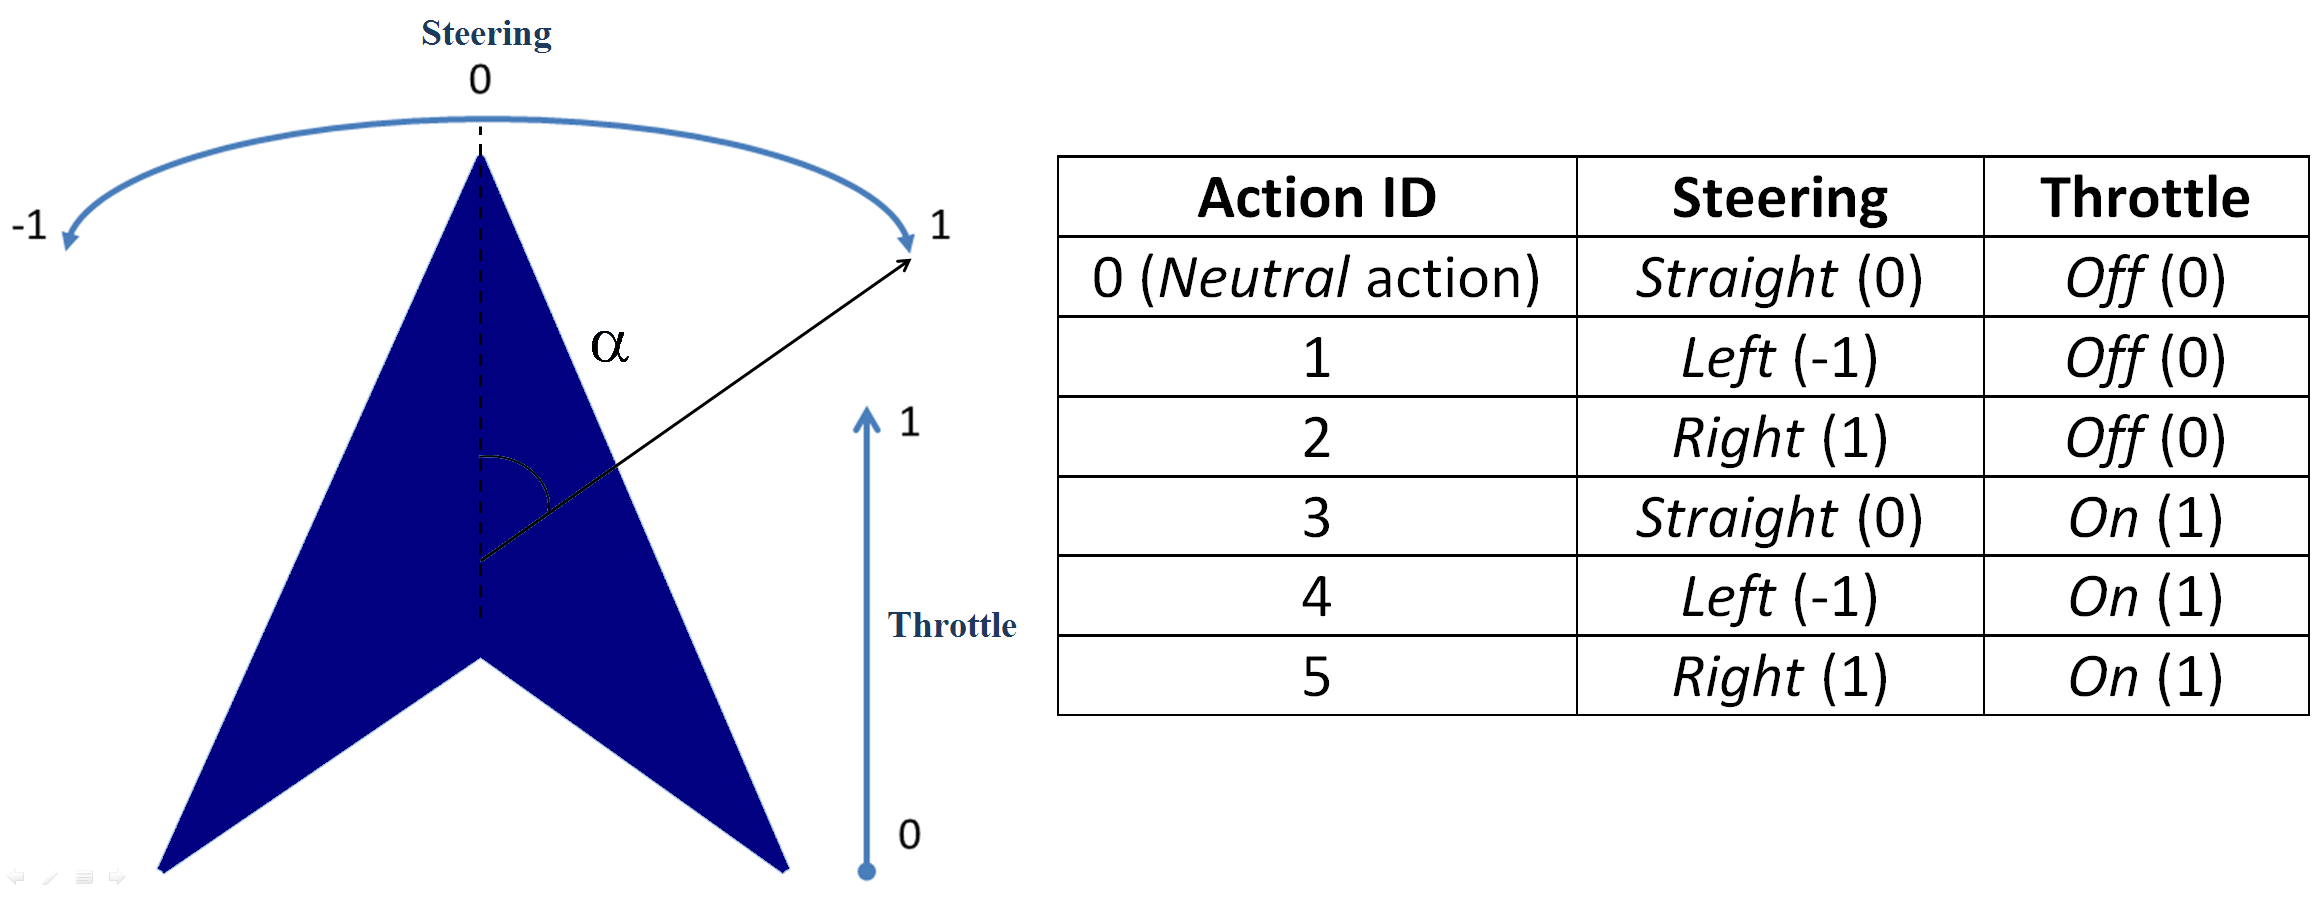
\includegraphics[scale=0.14]{img/ShipActions}
	\caption{Ship inputs and actions.}
	\label{fig:ship}
	\end{center}
\end{figure}

Left and right rotations are performed using a single angle, set to $\pi/60$ radians, and ship speed is set to $0.025$ pixels per time step, values determined by trial an error in order to provide a satisfactory game-play experience. The ship keeps its velocity from a game state to the next, making \textit{inertia} a key aspect to take into account when governing the ship. However, the ship would reach a full stop eventually if no acceleration actions are provided, as there is a loss of speed due to \textit{friction}. This friction is  set to $0.99$ (this is, only $1\%$ of the speed is lost at each step), a value also determined empirically. Finally, there is also a speed gain for actions with throttle on, which is set to $0.025$ pixels per game step. 

The location of the ship in the world can be uniquely determined by three vectors: \textit{position}, that specifies the coordinates of the center of the ship in the maze; \textit{direction}, a vector that indicates where the ship is pointing at (in other words, indicates the direction of a front vector); and \textit{velocity}, that determines the movement of the ship, including its direction and speed. Note that direction and velocity do not need to be aligned. Given an action, this part of state of the ship is modified as shown in Algorithm~\ref{alg:shipUpadte}.

\begin{algorithm}[!h]
\begin{algorithmic}
\Function{ShipUpdate}{$action$}
	\State $throttle \gets action.\Call{GetThrottle()}{}$
	\State $steering \gets action.\Call{GetSteering()}{}$

	\State $ship.direction.\Call{Rotates}{steering \times steerStep}$

	\If{$throttle == true$}
		\State $ship.velocity.\Call{Add}{ship.direction \times shipSpeed}$
	\EndIf

	\State $ship.velocity.\Call{Multiply}{frictionLoss}$
	\State $ship.position \gets ship.position + ship.velocity$


\EndFunction
\end{algorithmic}
\caption{Ship update function - no collisions.}
\label{alg:shipUpadte}
\end{algorithm}

The ship can also hit obstacles while it moves within the level, so position and velocity need to be updated differently if the ship's circular bounding collision hits a obstacle in the maze. When this happens, speed is reduced (by a $75\%$ factor) and the velocity vector is modified so the ship bounces off the wall with the appropriated angle. However, the MO-PTSP game introduces a new type of \textit{elastic} obstacle. In the case when the ship hits this kind of obstacle, the reduction of the speed is minor (only $10\%$), so the player can use this type of walls to change direction of travel abruptly without losing too much speed. A third type of obstacle (known as \textit{damaging} obstacle), produces a more important decrease in the speed of the ship, reducing it by a factor of $90\%$.

Another similarity between PTSP and MO-PTSP is the real-time component of the game: the player (also referred here as the agent, or the controller) must supply an action within a limited budget time, set to $40$ milliseconds. This limitation forces the controller to determine the next move quickly, rewarding those agents that are able to plan faster and explore the action search space in a more efficient manner.

While the PTSP was a bit more permissive, MO-PTSP imposes disqualifications in case this time limit is severely violated. In the original game, a neutral action was applied if the controller took more than $40$ milliseconds to provide an action, but no other consequences were derived from this misbehaviour. The game was then susceptible to cheating, as an agent could employ as long as it needs to plan ahead while the only consequence would be a neutral action in a single game tick. 

MO-PTSP tackles this situation by imposing a second time limit, set to $120$ milliseconds so, in case it is violated, produces the end of the game by disqualifying the player. Although controllers could still potentially spend more than $40$ milliseconds (with the same neutral move performed as a penalization), the risk of being disqualified and the limited gain that could be obtained by these extra milliseconds up to $120$ discouraged participants to performed this trick.

\subsection{A Multi-Objective Approach}

The main difference with respect to the original game, the PTSP, can be found in the three different objectives that need to be minimized:

\begin{itemize}
\item Time: the player must collect all waypoints scattered around the maze in as less time steps (or game cycles) as possible.
\item Fuel: the fuel consumed at the end of the game must be minimized.
\item Damage: the ship should end the game with as little damage as possible.
\end{itemize}

It is very important to stress that all waypoints must be visited in order to consider a game as successfully finished. Otherwise, a very simple but plausible approach for the player can be not to move at all and hence obtain a good result for the other two objectives (no fuel spent and damage suffered). A time dependant game over condition is established when the ship does not visit a waypoint once a timer has run off. This timer, initially set to $800$ time steps, is reduced by $1$ at every step if no waypoint is visited, causing the end of the game if it gets to $0$\footnote{PTSP also employed this timer, starting at $1000$. Hence, MO-PTSP is slightly more difficult in this sense, as it requires faster controllers.}. 

The ship starts with an initial fuel of $5000$ units, and one unit is spent every time an action with the throttle input set to \textit{on} is performed. The player adds, however, $50$ more units to the ship's fuel tank every time a waypoint is visited. Also, four \textit{fuel canisters} are also scattered around the maze, that provide $250$ units of fuel. It is important to mention that it is not mandatory to pick these fuel canisters up in order to complete the game, being their collection up to the strategy of the player. In case the amount of fuel available in the ship gets to $0$, the agent will not be able to use the throttle any more. 

Regarding the third objective, the ship can be damaged by two different game play elements. First, lava lakes are present in the game levels, dealing $1$ unit of damage for every game step the ship is flying over them. Secondly, the ship also gets damage when colliding with (non-elastic) obstacles, such normal and \textit{damaging} obstacles. The former type of obstacles (normal walls, also present in the PTSP game) inflict $10$ units of damage. The latter obstacles, created for this game, produce a more harming effect, dealing $30$ damage units. If the player's damage gets up to $5000$ units, the ship is destroyed and the game is over.

When the ship is damaged by a collision, it enters in an invulnerable state, where no more collision damage can be dealt to the agent (although lava still affects the ship) during $50$ game steps. This avoids situations when too much damage is suffered by the ship if it is touching an obstacle right after colliding with it.

\section{The MO-PTSP Competition}

\todo[inline]{Infrastructure of the competition, rules, how entries are ranked.
Evaluation, submission, programming specification, API.
Sample controllers: random, greedy, macro-action random search controller. Include some measurements.}

\section{The winning entry}

\todo[inline]{YORK DESCRIPTION.}

\section{Results of the competition}

\todo[inline]{Describe results in detail.}

\section{Conclusions}

\todo[inline]{We had lots of fun.}

\bibliographystyle{IEEEtran}
\bibliography{IEEEabrv,biblio}

\end{document}
